% $Id: CONTENT.tex 11855 2010-08-17 14:52:50Z alexandra $
% Local Variables:
% ispell-check-comments: nil
% Local IspellDict: american
% End:
% --------------------------------------------------------
% User documentation
% copyright by BREDEX GmbH 2005
% --------------------------------------------------------
% this command can be inserted multiple times
%\gdhelpid{}
% 
%\begin{gddescription}
%\end{gddescription}
%
%\begin{gdlist}
% use the \item command for single steps
%\end{gdlist}
% change <PATH> to the same directory, file is located in
% change <FILE> to the same filename you are editing
%\bxinput{<PATH>/Links/<FILE>}
%
% other usefull commands are
%   \bxtipp{}        to create a hint
%   \bxwarn{}        to describe a warning

The amount of keywords you have in a \app{} test and the amount of components your test deals with can grow very quickly. For this reason, it is important to think about structuring the \gdtestcasebrowser{} and the \gdomeditor{} to make finding \gdcases{} and component names easier. 


\subsection{Creating new component names}
\gdhelpid{guidancerComponentNameBrowserContextId}{Component Name Browser}
\gdhelpid{objectMapEditorContextId}{Object Mapping}
\gdhelpid{newComponentNameContextId}{New Component Name Dialog}
\label{TasksCreateNewCompName}
\index{New!Component Name}
\index{Add!Component Name}
\index{Component!Names!New}

For information on creating new component names by \bxname{reassigning} old component names (in the \gdcompnamesview{} for example, see the section on reassigning component names \bxpref{TasksReassignCompName}. 

You can create new component names in the \gdcompnamebrowser{}  and in the \gdomeditor{} (tree view) via the context menu:\\
\bxmenu{New Component Name}{}{}

\bxtipp{You can also use the toolbar button to create a new component name when you are in the \gdomeditor{}.}

A dialog will appear to allow you to enter a component name. We recommend having good naming conventions for component names, as this will help you when mapping later. 

The component name you enter will be created and will appear in the \bxname{unassigned component names} category in the \gdomeditor{} and in the \bxname{unused component names} category in the \gdcompnamebrowser{}. 

\bxtipp{Newly created component names have the type \bxname{graphics component} until they are made more specific, either by mapping them to a technical name or by entering this new name in the \gdcompnamesview{} for a more concrete component type. }


 
\subsection{Entering and reassigning component names in the \gdcompnamesview{}}
\gdhelpid{compNameViewContextId}{Component Names View}
\label{TasksReassignCompName}
\index{Component!Names!Reassigning}
\index{Reassigning!Component Names}
\index{View!Component Names}
\index{Component!Names!View}
\index{Names!Component!Reassigning}
\index{Component!Names!Local}
\index{Component!Names!Global}
\index{Local Component Names}
\index{Global Component Names}
\index{Component}

\bxtipp{The following section deals with entering component names in the \gdcompnamesview{} when you have added \gdcases{} from the library. For information on component names in \gdsteps{}, see the \gdsteps{} section \bxpref{specsteps}.}

\begin{enumerate}
\item Once you have added a \gdcase{} from the library of \gdcases{}, you will need to enter a component name for the component you want to test. 
\item In the \gdcompnamesview{}, you will see the \bxname{old name} for this component, which was given in the \gdstep{} contained in the library \gdcase{}. The old name is just a placeholder and should be \bxname{reassigned} (\bxfigref{compnamesview}).

\begin{figure}[h]
\begin{center}
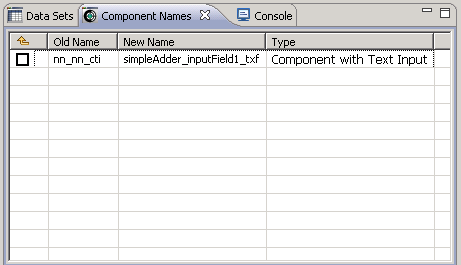
\includegraphics{Tasks/Compnames/PS/compnamesview}
\caption{The \gdcompnamesview{}}
\label{compnamesview}
\end{center}
\end{figure} 
 

\bxtipp{Reassigning component names: by entering a different component name in the \gdcompnamesview{} you create a new reference to a component in the \gdaut{}. You can create as many new component names as you like for each \gdcase{}. This lets you execute the same actions on different (but compatible) components without having to specify whole new \gdcases{} to do this. Reassigning is different to \bxname{renaming} - whereby you simply change the name of a reference to a component \bxpref{TasksRenameCompName}. }

\item In the \bxname{new name} field, enter your name for this component, e.g. \bxshell{MainWindow\_NavigationTree\_tre}. 

We recommend using naming conventions for component names \bxpref{BPComponentNames}. 

\item Press \bxkey{Ctrl+SPACE} to see a list of component names you have already used for this type of component:

\begin{description}
\item[\bxname{Local}]{ component names are names you have used in this \gdcase{} for this component type. }
\gdmarpar{../../../share/PS/localName}{Local name}
\item [\bxname{Global}]{ component names are names you have used for this component type, but not in this \gdcase{}. }
\gdmarpar{../../../share/PS/globalName}{Global name}
%\item [Unused]{ component names are names that have already been mapped to this component type in the \gdaut{}. The \gdcase{} containing the component name has since been deleted.}
% \gdmarpar{../../../share/PS/OMLogName}{unused name}
 \end{description}

\item The component name you enter here will be collected by the \gdomeditor{} when you carry out object mapping so that you can assign it to a component in the \gdaut{}. 

\item Every time you want to carry out an action on this component, use this name. 
\end{enumerate}
\bxtipp{See the section on the component hierarchy for some tips on using component names in your tests \bxpref{TasksCompNameType}.}

\subsubsection{Writing \gdcases{} that can test different components in the \gdaut{}}
\gdhelpid{compNameViewContextId}{Component Names View}
\label{TasksCompNamesCheckbox}
Select the checkbox on the left of the \gdcompnamesview{} to be able to see and edit (reassign) this component name when you reuse the parent of the \gdcase{} you are editing. 

This is useful for creating flexible keywords that can click either the cancel button or the ok button in a dialog, for example. Depending on what you want the keyword to do when you reuse it, you can overwrite the name to \bxname{LoginDialog\_OK\_btn} or \bxname{LoginDialog\_Cancel\_btn}. 

\subsubsection{Changing component names}
If you newly reassign component names in  your test hierarchy that were themselves later reassigned, you will be shown a message in the \gdcompnamesview{}.
\begin{itemize}
\item The message only appears at places where you have reused the \gdcase{} containing that component, and where you have overwritten the component name. 
\item For example:
\begin{enumerate}
\item Your component was originally called \bxname{LoginDialog\_nn\_btn}.
\item You reused the \gdcase{} containing this component, and renamed the component \bxname{LoginDialog\_OK\_btn}.
\item You then change the component name in the original \gdcase{} to \bxcaption{LoginDialog\_AnyButton\_btn}.
\end{enumerate}
\item In the \gdcompnamesview{} for the reused \gdcase{}, you will see a warning message that the component name has no type.
\item You will also see the new name for the component.
\bxwarn{The warning field is not editable.}
\item If you want to keep the same overwritten name, enter the name into the \bxcaption{new name} field in the row for the new component name.
\item You can also change the overwritten name, or not overwrite it at all. In this case you will need to adapt your object mapping, if this component has been used in a \gdsuite{}. 
\item Once you have saved the \gdcompnamesview{}, the warning message will disappear. 
\end{itemize}


\subsection{Renaming component names}
\gdhelpid{guidancerComponentNameBrowserContextId}{Component Name Browser}
%\gdhelpid{objectMapEditorContextId}{Object Mapping}
\gdhelpid{renameComponentNameContextId}{Rename Component Name Dialog}
\label{TasksRenameCompName}
\index{Test Case!Renaming}
\index{Renaming!Test Cases}
\index{Test Suite!Renaming}
\index{Renaming!Test Suites}
\index{Test Job!Renaming}
\index{Renaming!Test Jobs}
\index{Renaming!Component Names}
\index{Component Name!Renaming}

To rename an item in the \gdtestcasebrowser{}, \gdtestsuitebrowser{} or \gdcompnamebrowser{}:

\begin{enumerate}
\item Select the item you want to rename in the browser. 
\item Select:\\
\bxmenu{Rename}{}{}\\
from the context-sensitive menu. 
\item In the dialog which appears, enter a new name and click \bxcaption{OK}. 
\end{enumerate}

\bxtipp{You can also press \bxkey{F2} to rename an item.}

When you rename a \gdcase{} or \gdsuite{}, you change its specification name. 

If you have reused this \gdcase{} or \gdsuite{} in other \gdcases{}, \gdsuites{} or \gdjobs{}, the name will also be changed in the places where you have reused it but not renamed it. 


\subsection{Merging component names}
\gdhelpid{guidancerComponentNameBrowserContextId}{Component Name Browser}
\gdhelpid{objectMapEditorContextId}{Object Mapping}
\gdhelpid{mergeComponentNameContextId}{Merge Component Name Dialog}
\label{TasksMergeCompName}
\index{Component!Names!Merge}
\index{Merge Component Names}

You can merge two or more component names to one unifying name in the \gdomeditor{} (tree view) and in the \gdcompnamebrowser{}. This makes sense if you have accidentally created two component names for the same component. 

\bxtipp{The component types must be the same to be able to merge the component names, and the component names must not have already been mapped to different technical names from the \gdaut{}. The component names must all come from the current \gdproject{}, not from any of the reused \gdprojects{}.}

To merge component names:
\begin{enumerate}
\item Select the component names you want to merge. Use \bxkey{CTRL} to select multiple names. 
\item From the context-menu, select:\\
\bxmenu{Merge Component Names}{}{}
\item A dialog will appear in which you can choose which of the selected names you want to merge all the names to. Select the name you want and click \bxcaption{OK}. 
\item The component names you selected will be merged to the name you specified throughout your test. 
\end{enumerate}


\subsection{Deleting unused component names}
\gdhelpid{guidancerComponentNameBrowserContextId}{Component Name Browser}
\label{TasksDeleteCompName}
\index{Component!Names!Delete}
\index{Delete!Component Names}

When you reassign component names in the \gdcompnamesview{}, you automatically create new component names if the name you enter did not previously exist in the \gdproject{}. 

Larger \gdprojects{} can often end up with a number of component names that are no longer used. You can see and delete these names in the \gdcompnamebrowser{}. 
The names in the \bxname{Unused Component Names} category are not used anywhere in this \gdproject{} -- they are not present in any \gdcases{} and they have not been mapped to any technical names from the \gdaut{} in the \gdomeditor{} (\bxfigref{}). 

\begin{figure}[h]
\begin{center}
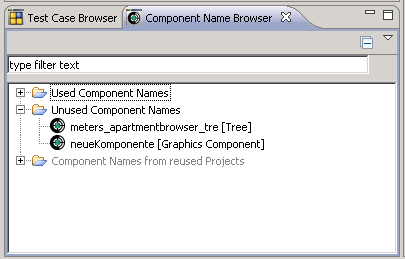
\includegraphics{Tasks/Compnames/PS/compnamebrowser}
\caption{The \gdcompnamebrowser{}}
\label{compnamebrowser}
\end{center}
\end{figure} 

To delete unused component names, select the name you want to delete and select:\\
\bxmenu{Delete}{}{}\\
from the context-menu. 



\subsection{Understanding the component hierarchy}
\gdhelpid{guidancerComponentNameBrowserContextId}{Component Name Browser}
\gdhelpid{compNameViewContextId}{Component Names View}
\gdhelpid{objectMapEditorContextId}{Object Mapping}
\label{TasksCompNameType}
\index{Component!Names!Hierarchy}
\index{Hierarchy of Component Names}
\index{Abstract components}
The component hierarchy in \app{} is designed to allow flexible test specification and robust tests. For a graphical overview of the component hierarchy, see the reference manual \bxextref{\gdrefman}{ref,overviewabstcomp}. 
\bigskip

\textbf{Abstract components}\\

\app{} lets you write tests very abstractly at the beginning, only adding detail later. You will notice that the library contains categories such as \bxname{Component with Text Input} and \bxname{Graphics Component}. 

These are \bxname{abstract components} -- actions in these categories can be used on a wide range of actual components in the \gdaut{}. You can use a \bxname{Click} action on the \bxname{Graphics Component} to click any component in the \gdaut{}. You just need to enter different component names for it in the \gdcompnamesview{}. 
\bigskip
\textbf{Using the same component name for different component types}\\

What happens if you want to specify a test that clicks in a table and then selects a cell in the table?

The click action is on the \bxname{Graphics Component} and the select cell action is on the \bxname{Table} component -- but you don't want to have two different component names. 

This isn't a problem for \app{}. You can use the same component name for different components as long as these are compatible. So, in this case, the \bxname{Graphics Component} and the  \bxname{Table} component can both use the component name \bxname{TableView\_MainTable\_tbl}. 

\bxwarn{You cannot use the same component name for incompatible types, for example, trees and tables.}

An overview of the component hierarchy can be seen in: \bxextref{\gdrefman}{ref,overviewabstcomp}.

